% Slides for 2024-07-30
% To create a slide, use the following:
% \begin{frame}{TITLE}
%     BODY
% \end{frame}

% To create a slide with a bullet list, use the following:
% \begin{frame}{TITLE}
%     \begin{itemize}
%         \item ITEM 1
%         \item ITEM 2
%     \end{itemize}    
% \end{frame}

% To create a slide with numbered list, use the following:
% \begin{frame}{TITLE}
%     \begin{enumerate}
%         \item ITEM 1
%         \item ITEM 2
%     \end{enumerate}
% \end{frame}

% To create a slide with a graphic:
% 1. Add the graphic to this folder (named picture.png)
% 2. Use the following:
% \begin{frame}{TITLE}
%     \centering
%     \includegraphics[height=0.7\textheight,width=0.7\textwidth,keepaspectratio]{picture.png}
% \end{frame}

% To create a slide with two columns, use the following:
% \begin{frame}{TITLE}
%     \begin{columns}
%         \begin{column}{0.5\textwidth}
%             COLUMN 1 BODY
%         \end{column}
%         \begin{column}{0.5\textwidth}
%             COLUMN 2 BODY
%         \end{column}
%     \end{columns}
% \end{frame}

%% Announcements for 2025-06-20T14:00:00-07:00
% \begin{frame}{Announcements}
%     \begin{itemize}
%         \item
%     \end{itemize}
% \end{frame}

\begin{frame}{Edge Contraction}
    \begin{center}
        Previous Mesh
    \end{center}
    \begin{center}
         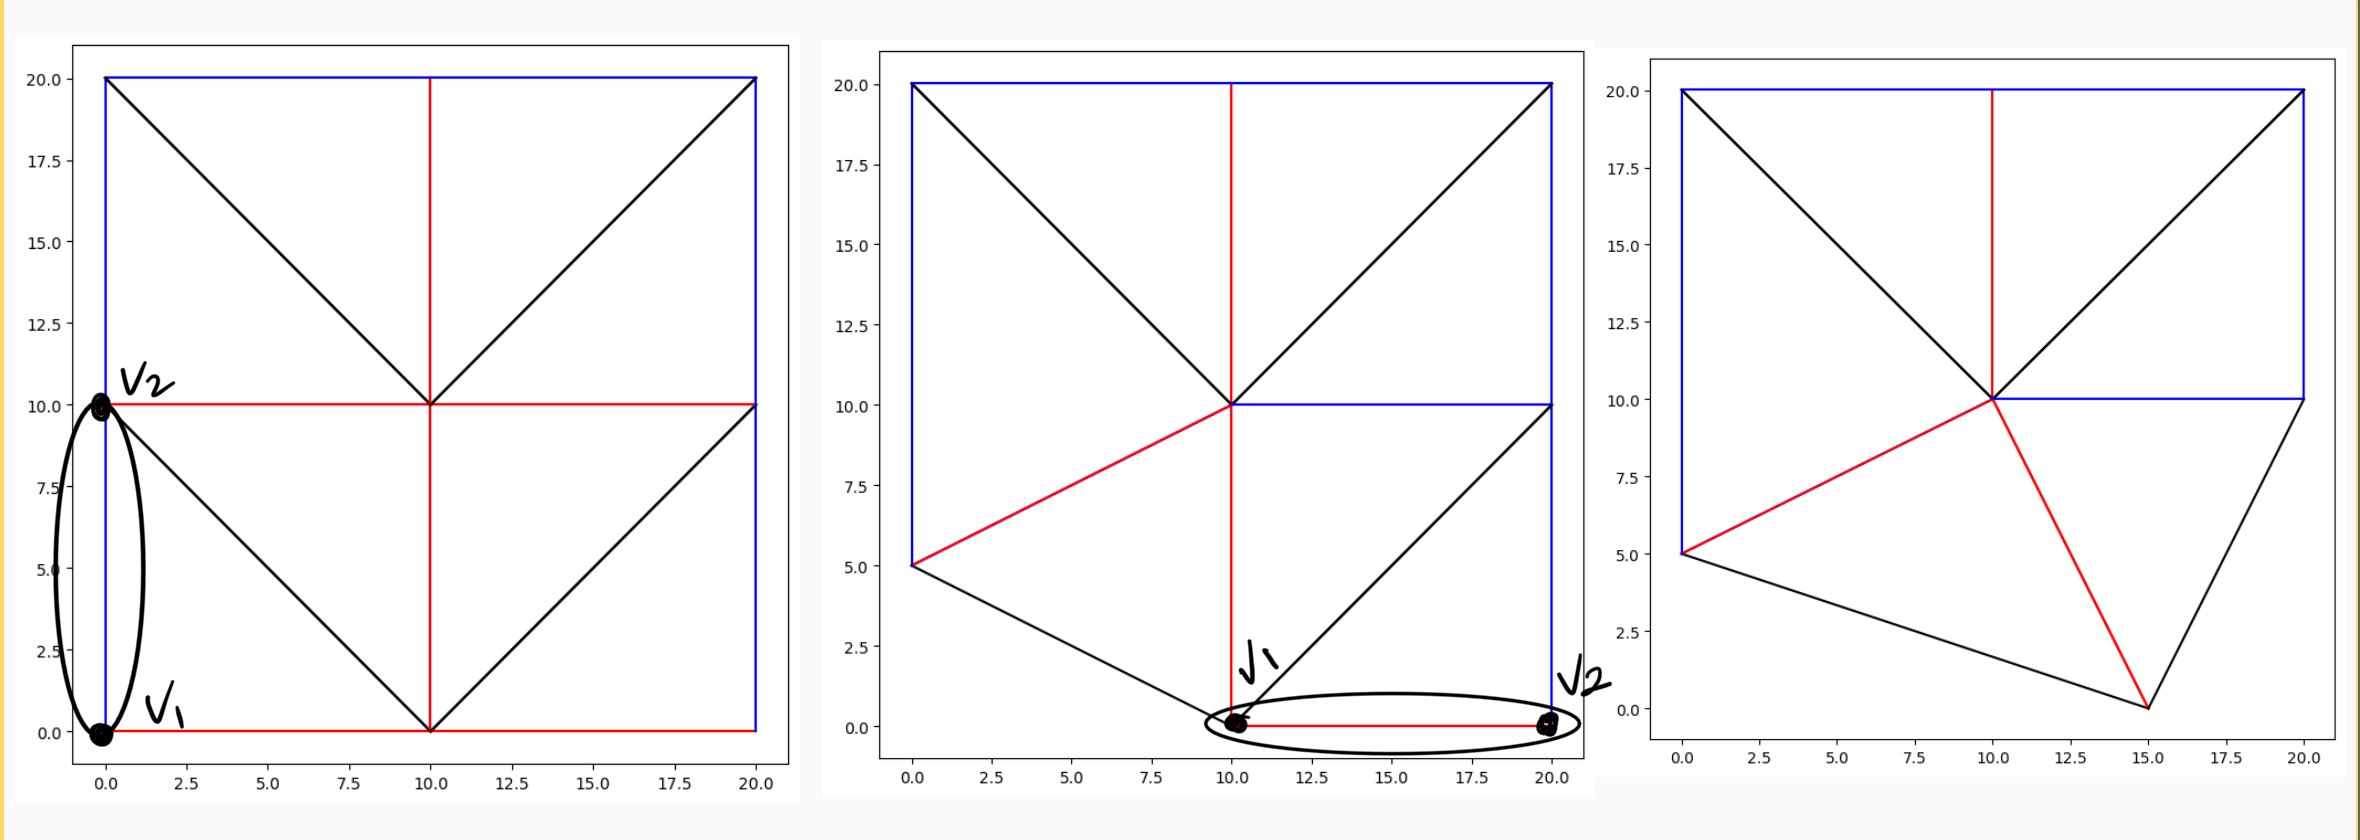
\includegraphics[scale=0.17]{images/testdata.jpg}
         
         
    \end{center}
   

\end{frame}
\begin{frame}{Fixing Errors}
\begin{center}
    
        Current Mesh
        
    \end{center}
    \begin{center}
        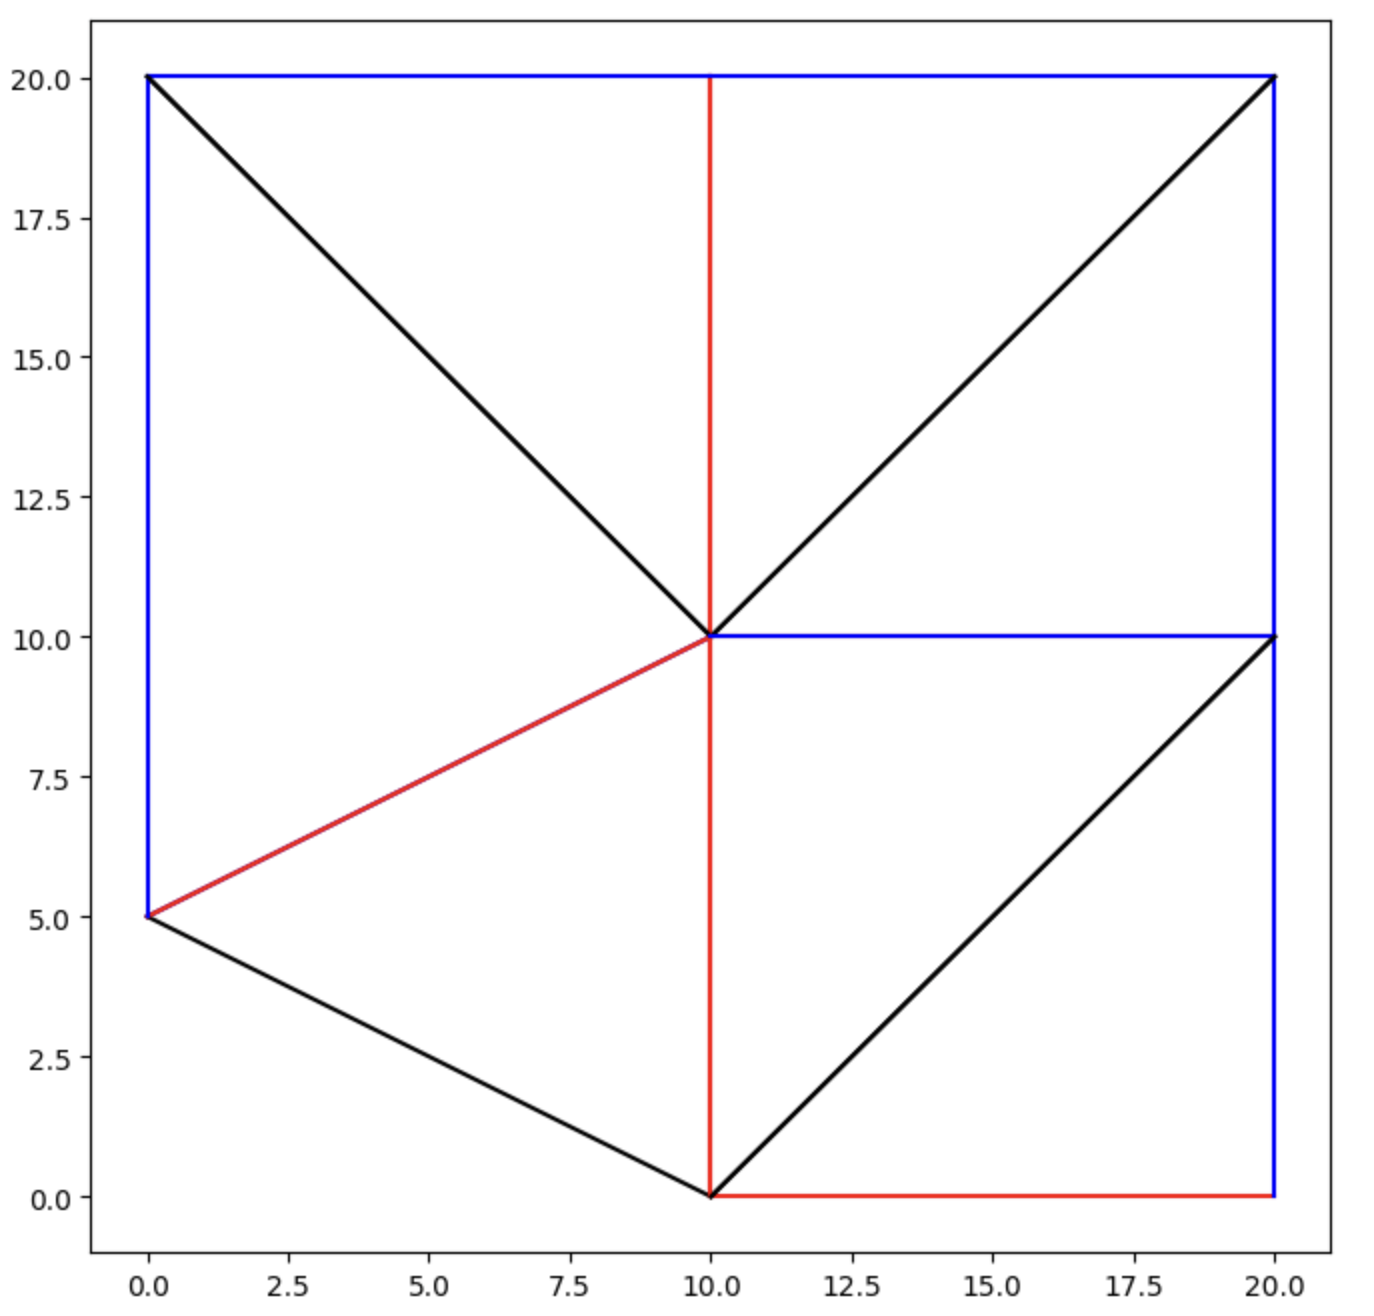
\includegraphics[scale=.18]{images/curr1.png}
         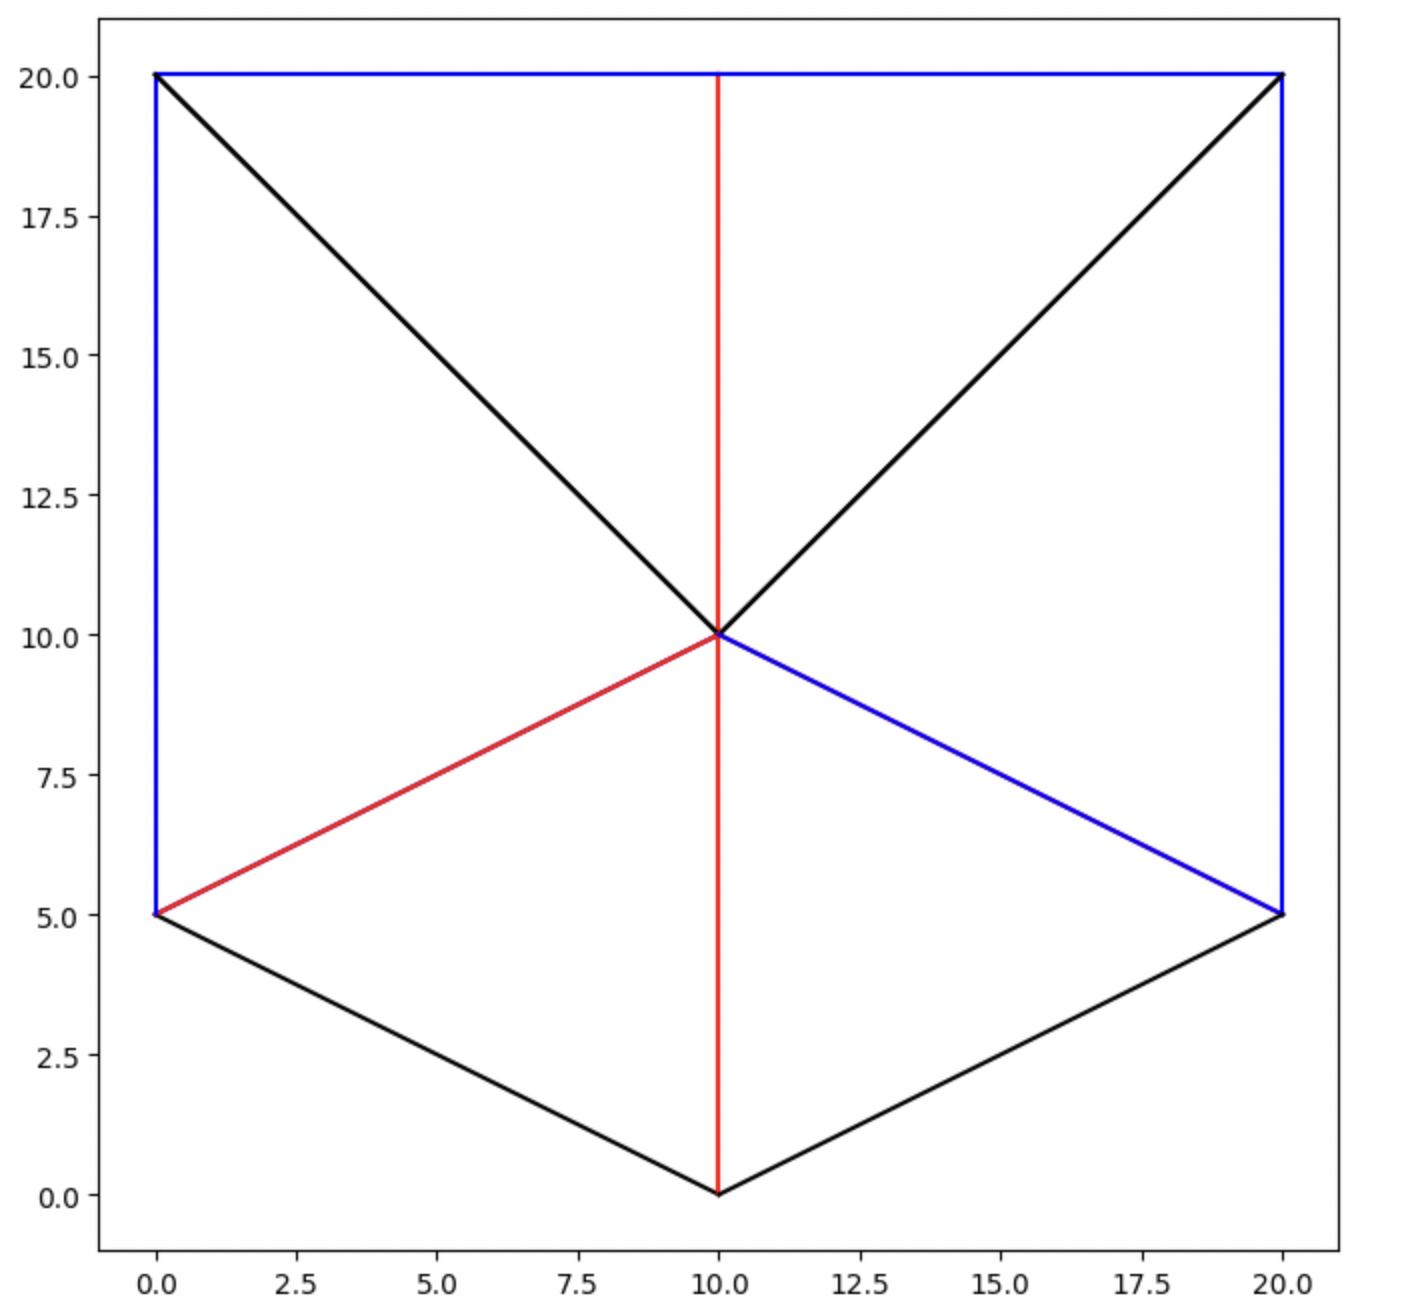
\includegraphics[scale=.18]{images/curmesh.png}
          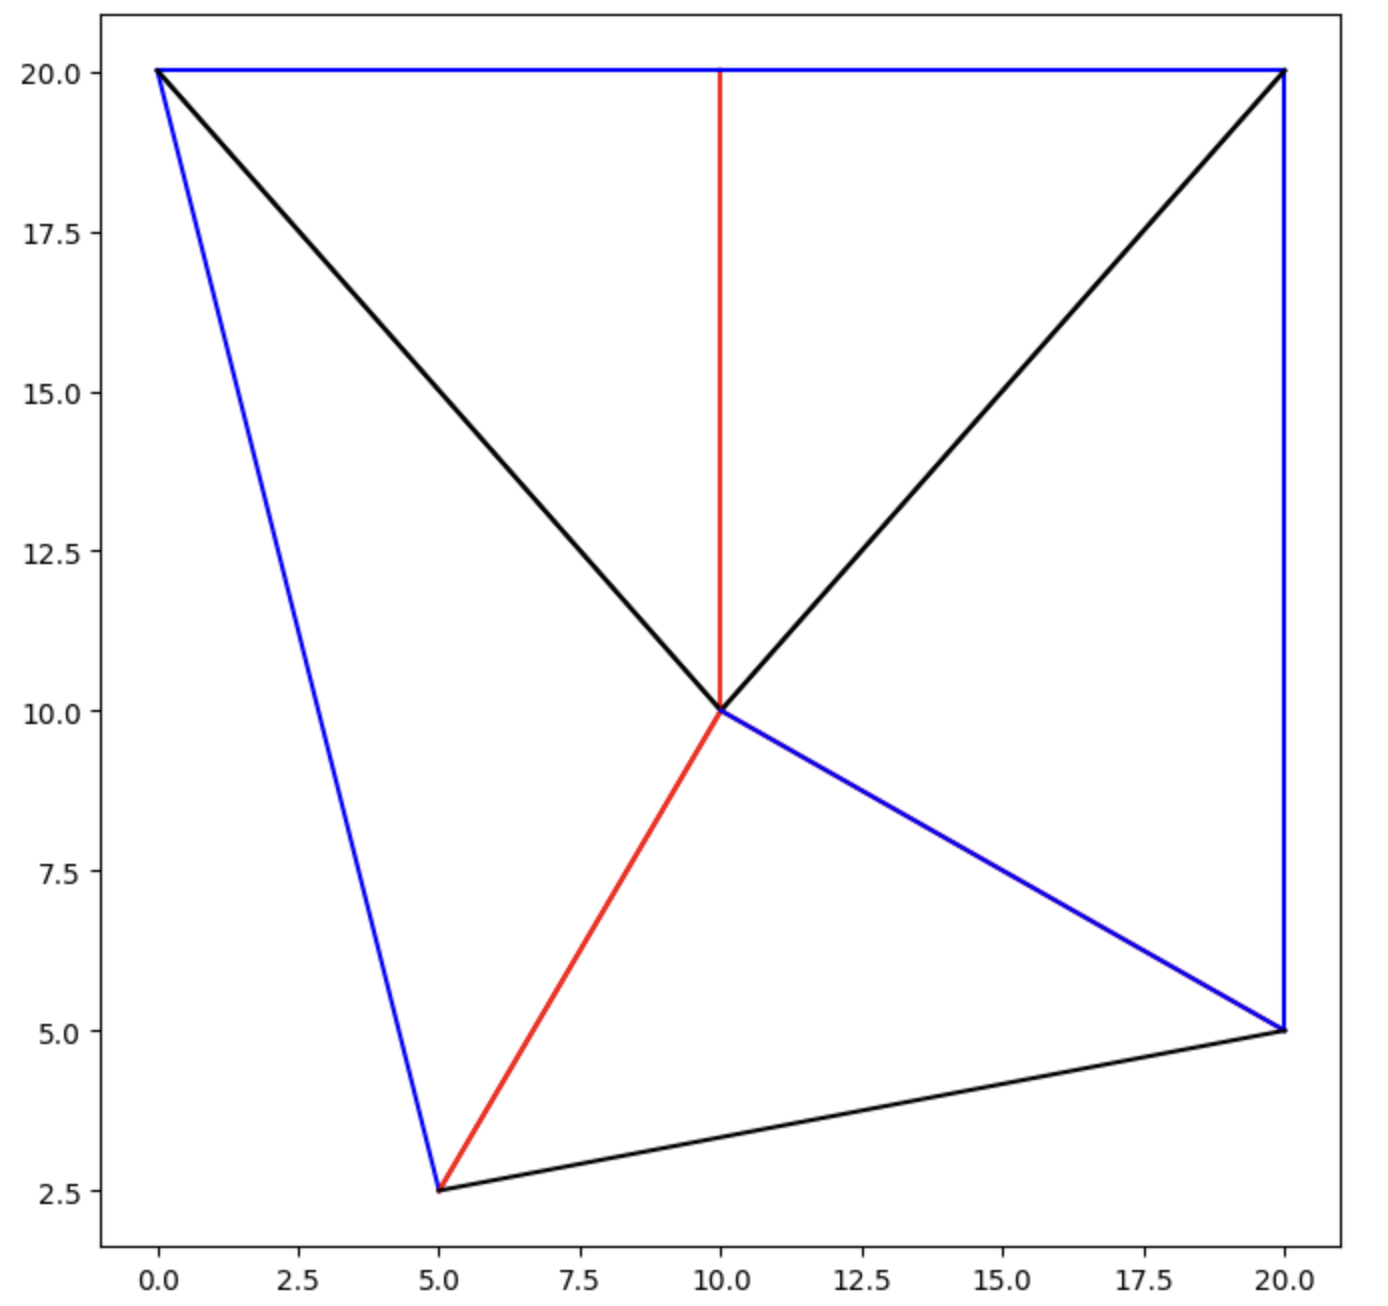
\includegraphics[scale=.18]{images/curr3.png}
        
    \end{center}

    
    

  
    

\end{frame}

\begin{frame}{Test Data}
\begin{center}
    
        50 by 50 grid
        
    \end{center}
    \begin{center}
        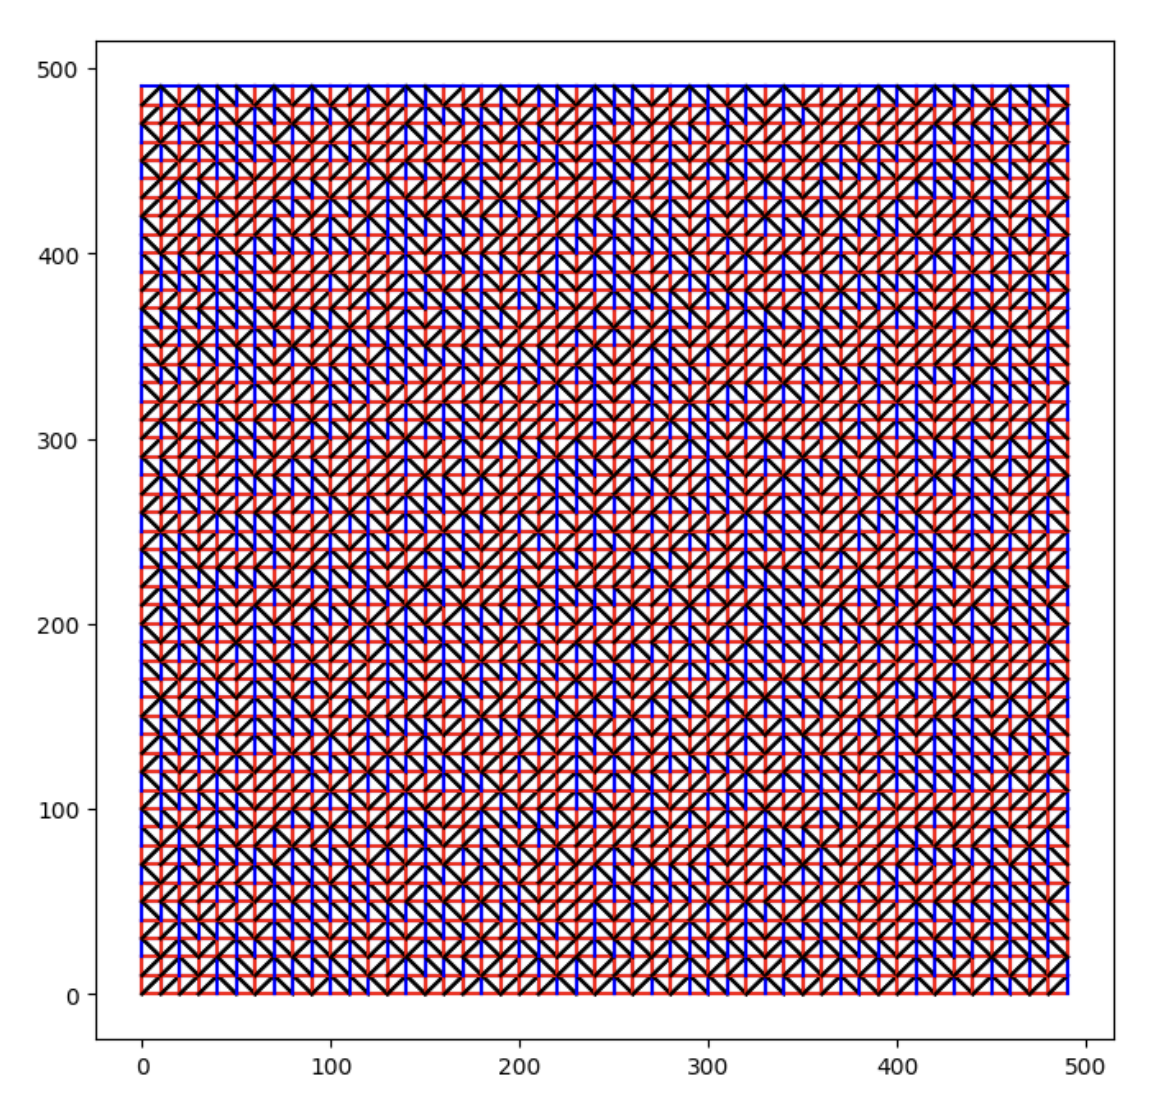
\includegraphics[scale=.3]{images/50by502d.png}
        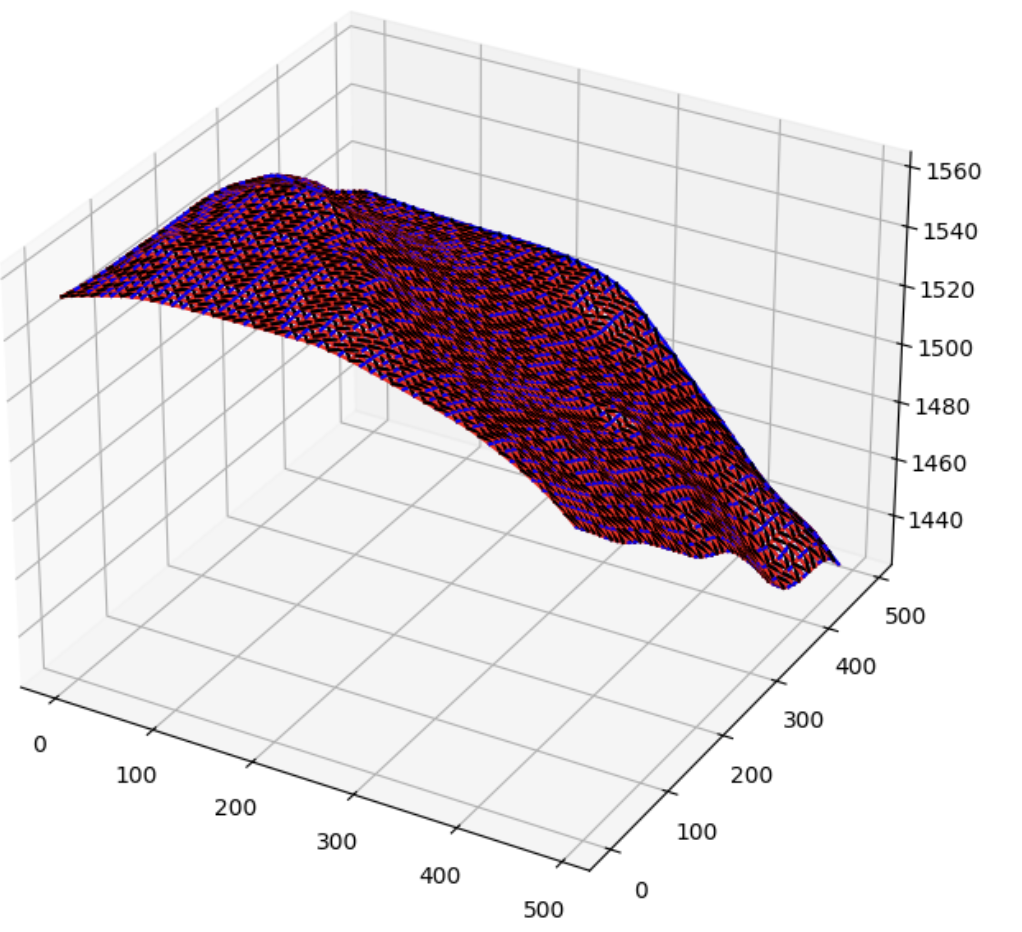
\includegraphics[scale=.36]{images/50by503d.png}
        
        
    \end{center}

\end{frame}

\begin{frame}{Test Data}
\begin{center}
    
        50 by 50 grid contracted
        
    \end{center}
    \begin{center}
        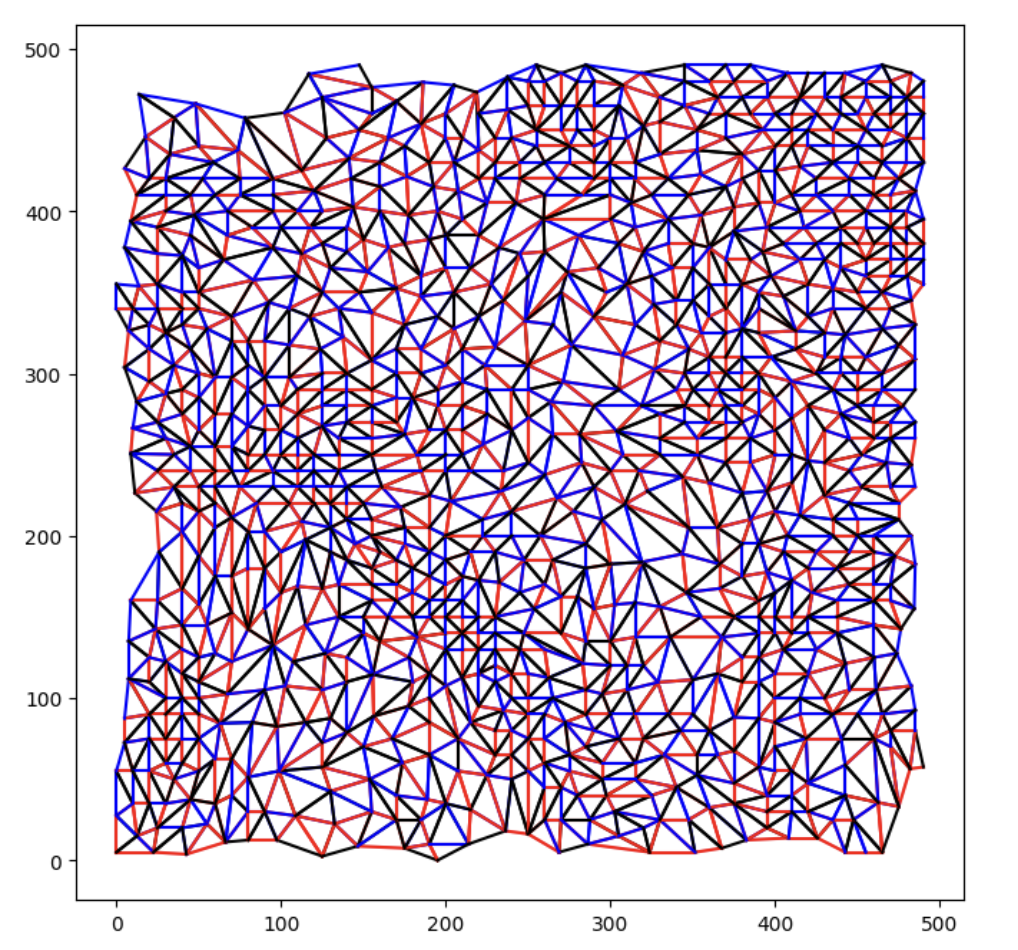
\includegraphics[scale=.36]{images/50by50contracted2d.png}
        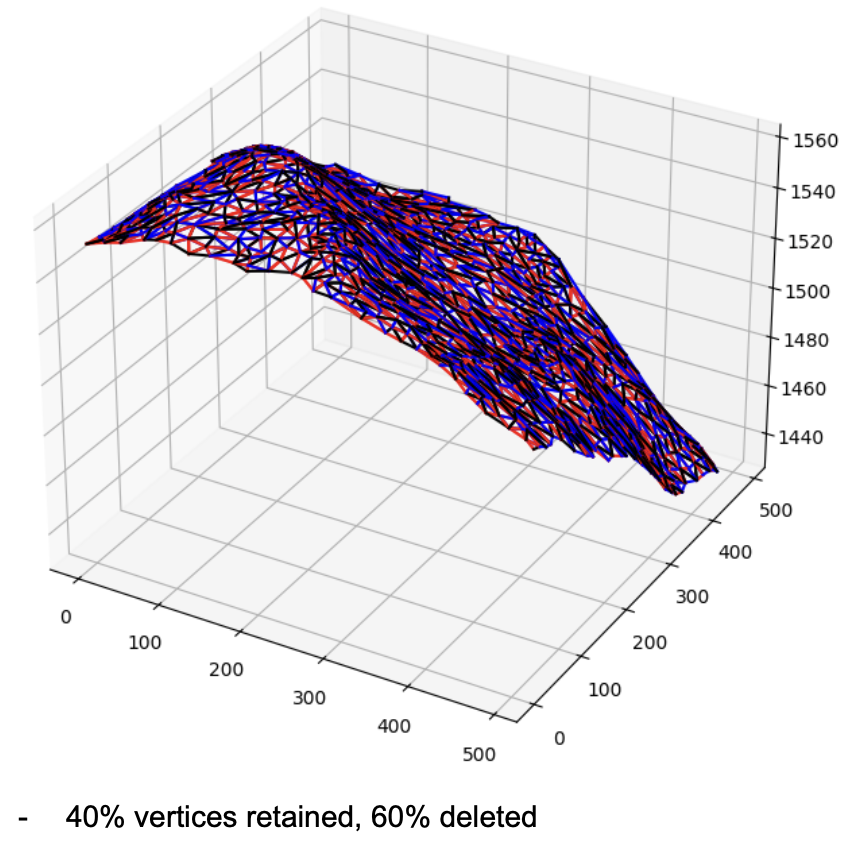
\includegraphics[scale=.4]{images/50by50contracted.png}
        
        
    \end{center}

\end{frame}

\begin{frame}{Test Data}
\begin{center}
    
        20 by 20 grid
        
    \end{center}
    \begin{center}
        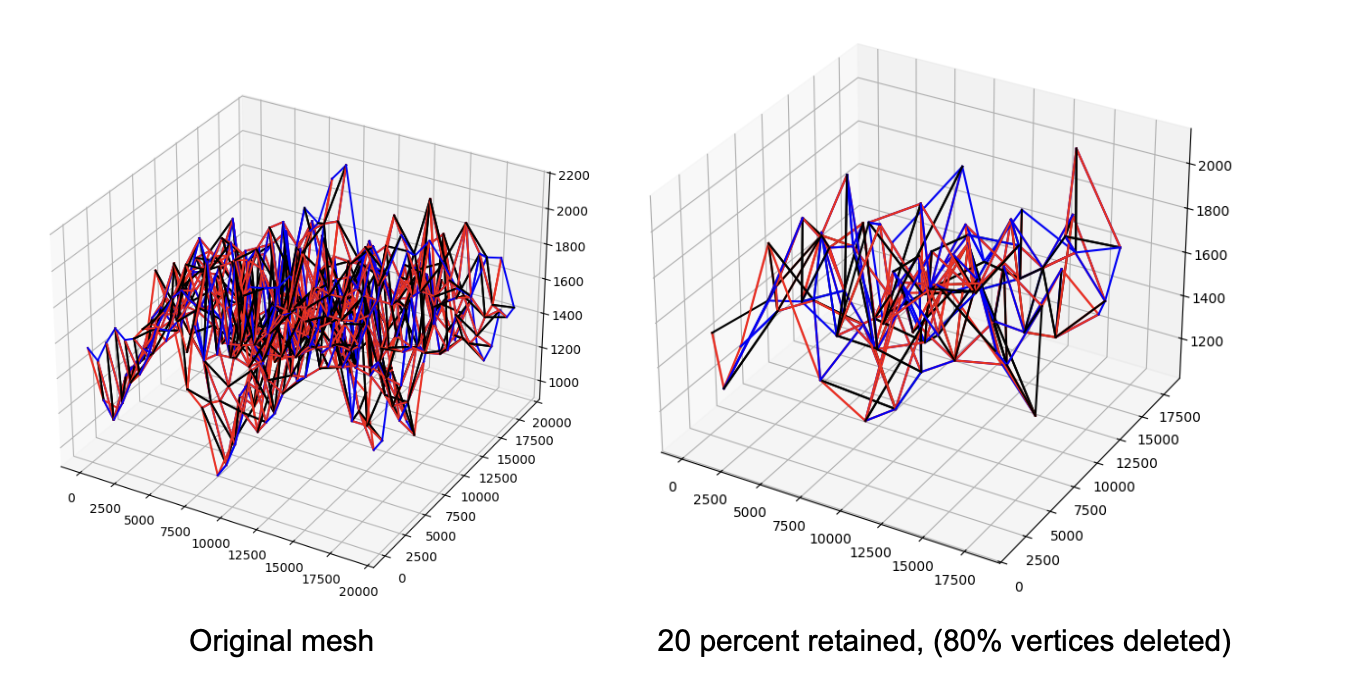
\includegraphics[scale=.58]{images/20by20.png}
        
    \end{center}

\end{frame}

\begin{frame}{Test Data}
    \begin{center}
        
            10 by 10 grid
            
        \end{center}
        \begin{center}
            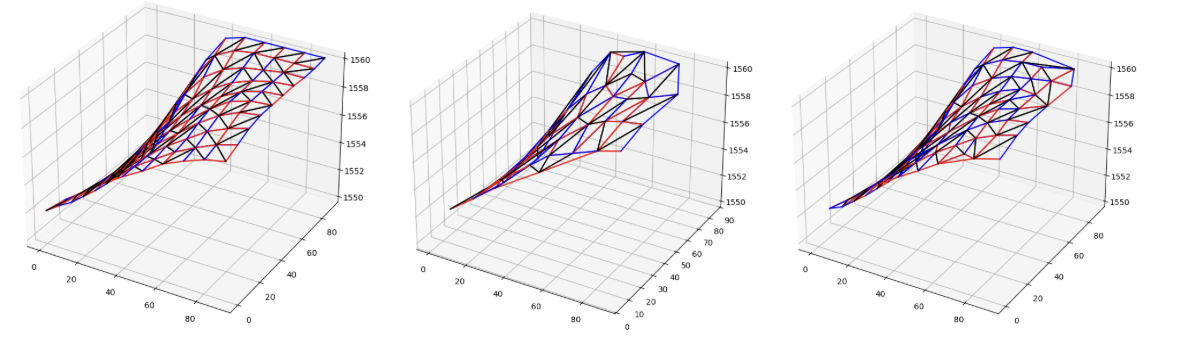
\includegraphics[scale=.74]{images/10by10.png}
            
        \end{center}
    
    \end{frame}